A continuación, se detalla la implementación técnica realizada en la topología de la empresa para dar cumplimiento a las nuevas políticas de seguridad solicitadas.



\subsection*{El Conflicto de Intereses}
Entendí que la Red A (Desarrollo: \texttt{192.168.10.0/24}) tiene prohibido iniciar cualquier tipo de comunicación hacia la Red B (Finanzas: \texttt{192.168.20.0/24}). Sin embargo, la Red B sí debe poder iniciar conexiones web (TCP puertos 80/443) hacia la Red A para ver sus herramientas de prueba.

Dado que necesitamos filtrar por origen, destino y tipo de conexión, decidí utilizar una Lista de Control de Acceso Extendida (ACL). El estándar indica que las ACL deben colocarse lo más cerca posible del origen del tráfico. Por lo tanto, la configuraremos en el router R-desarrollo en su interfaz Fa0/0.

Usaremos la palabra reservada \texttt{established} para TCP y \texttt{echo-reply} para ICMP. Esto permite que el tráfico de Desarrollo hacia Finanzas solo pase si es una respuesta a una petición que Finanzas pidió.

\begin{lstlisting}[language=bash, numbers=none]
	R-desarrollo> enable
	R-desarrollo# configure terminal
	
	- Permitimos que el tráfico TCP de Desarrollo a Finanzas pase solo si es una respuesta a una conexión ya establecida
	R-desarrollo(config)# access-list 110 permit tcp 192.168.10.0 0.0.0.255 192.168.20.0 0.0.0.255 established
	
	- Permitimos respuestas de ping
	R-desarrollo(config)# access-list 110 permit icmp 192.168.10.0 0.0.0.255 192.168.20.0 0.0.0.255 echo-reply
	
	- Bloqueamos cualquier otra comunicación IP que se inicie desde Desarrollo hacia Finanzas
	R-desarrollo(config)# access-list 110 deny ip 192.168.10.0 0.0.0.255 192.168.20.0 0.0.0.255
	
	- Permitimos que Desarrollo se comunique con cualquier otra red
	R-desarrollo(config)# access-list 110 permit ip any any
	
	- Aplicamos la ACL a la interfaz de la LAN de Desarrollo
	R-desarrollo(config)# interface FastEthernet 0/0
	R-desarrollo(config-if)# ip access-group 100 in
	R-desarrollo(config-if)# exit
\end{lstlisting}

\begin{figure}[H]
	\centering
	\vspace{-10pt}
	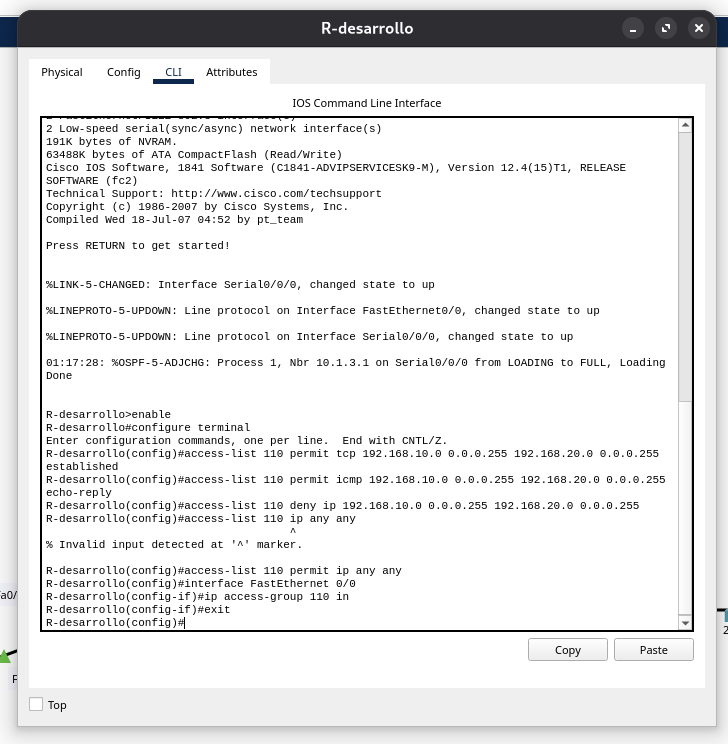
\includegraphics[scale=0.5]{imagenes/Capturas/11.png}
	\caption{Comandos en CLI del router Desarollo}
	\vspace{-20pt}
\end{figure}

Probamos la configuración en Cisco Packet Tracer:
\begin{itemize}
	\item En PC-dev hacemos un ping a la PC-finanzas (\texttt{ping 192.168.20.10}).  Nos debe rechazar la petición.
	\item En la PC-finanzas hacemos un ping a la PC-dev (\texttt{ping 192.168.10.11}). El resultado debe ser exitoso.
\end{itemize}

\begin{figure}[H]
	\centering
	 \begin{minipage}{0.3\textwidth}
		\centering
		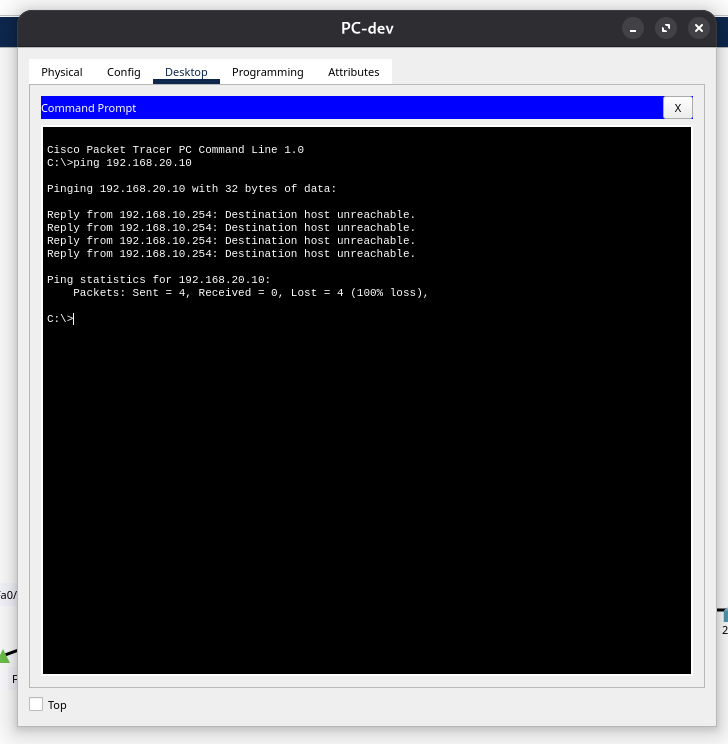
\includegraphics[scale=0.35]{imagenes/Capturas/12.png}
		\caption{Prueba en PC-dev}
	\end{minipage}
	\hfill
	\begin{minipage}{0.45\textwidth}
		\centering
		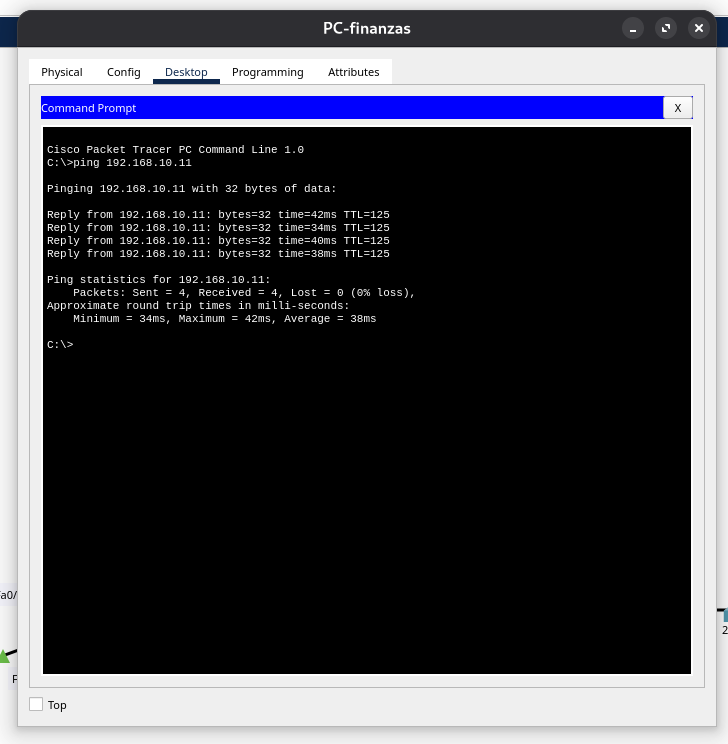
\includegraphics[scale=0.35]{imagenes/Capturas/13.png}
		\caption{Prueba en PC-finanzas}
	\end{minipage}
\end{figure}

\subsection*{Seguridad de la Infraestructura}
Entendí que la administración remota de los routers, por ejemplo, conexiones SSH o Telnet a través de las líneas virtuales o VTY, debe estar completamente bloqueada para todos los usuarios de la empresa, a excepción de una única IP específica: la de la PC-gerente (\texttt{192.168.10.10}).


Para proteger los accesos virtuales de un router, no se aplican las ACLs en las interfaces físicas (como Fa0/0), sino que decidí usar una Lista de Control de Acceso estándar (del 1 al 99) aplicada directamente sobre las líneas VTY (0 al 4 son las predeterminadas) mediante el comando \texttt{access-class}. Como esta es regla aplica para todo el negocio, \textbf{este paso debe repetirse exactamente igual en los 4 routers (R-desarrollo, R-finanzas, R-central, R-servidores)}.

\begin{lstlisting}[language=bash, numbers=none]
R-central> enable
R-central# configure terminal

- Creamos una ACL estandar que solo permita la IP del gerente
R-central(config)# access-list 10 permit host 192.168.10.10

- Ingresamos a las lineas virtuales del router
R-central(config)# line vty 0 4
R-central(config-line)# access-class 10 in

- Permitimos la conexion remota con SSH y Telnet
R-central(config-line)# transport input ssh
R-central(config-line)# transport input telnet
R-central(config-line)# exit
\end{lstlisting}

\begin{figure}[H]
	\centering
	\vspace{-10pt}
	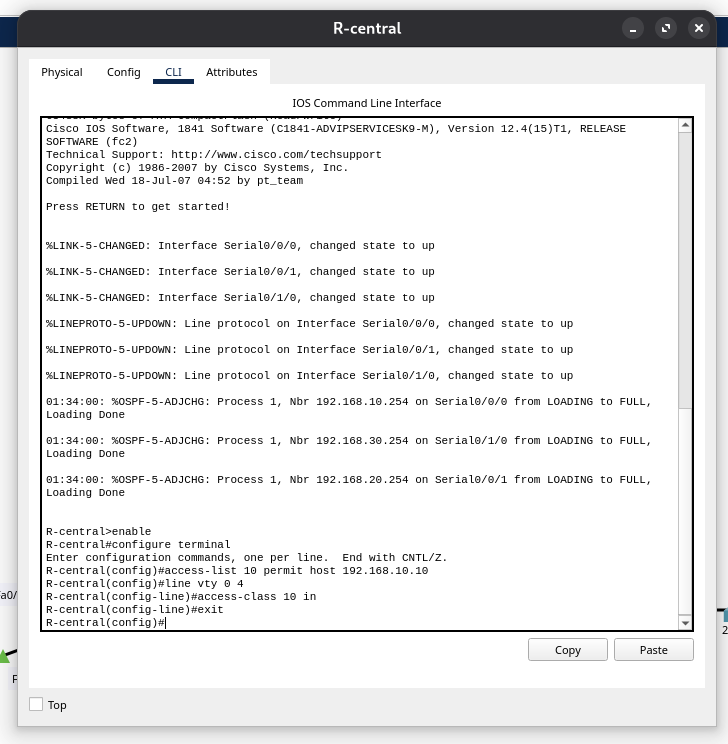
\includegraphics[scale=0.5]{imagenes/Capturas/21.png}
	\caption{Comandos en CLI para todos los routers}
	\vspace{-40pt}
\end{figure}

Sin embargo esta última configuración entro en conflicto con la del primer problema que ya se habia solucionado. Cuando desde la PC-gerente intenta hacer un Telnet (que es una conexión nueva TCP) hacia \texttt{192.168.20.254}, el paquete llega a R-desarrollo. El router revisa la ACL 110, ve que un equipo de la red \texttt{10.x} quiere ir a la red \texttt{20.x}, y rechaza el paquete, resultando en un \textit{Connection timed out} en lugar del login.

Esto se debe a que en las ACL, el orden importa. El router lee las reglas de arriba hacia abajo y realiza la acción de la primera coincidencia. Por lo tanto, tuve que modificar nuestra ACL 110 en R-desarrollo para poner una regla adicional para que el PC-Gerente (\texttt{192.168.10.10}) tenga permiso para pasar.

\begin{lstlisting}[language=bash, numbers=none]
	R-desarrollo> enable
	R-desarrollo# configure terminal
	
	- Borramos la regla anterior
	R-desarrollo(config)# no access-list 100
	
	- Permitimos que el gerente (192.168.10.10) vaya a donde quiera (any) para administrar
	R-desarrollo(config)# access-list 100 permit ip host 192.168.10.10 any
	
	- Volvemos a poner las reglas de la empresa en el mismo orden:
	R-desarrollo(config)# access-list 100 permit tcp 192.168.10.0 0.0.0.255 192.168.20.0 0.0.0.255 established
	R-desarrollo(config)# access-list 100 permit icmp 192.168.10.0 0.0.0.255 192.168.20.0 0.0.0.255 echo-reply
	R-desarrollo(config)# access-list 100 deny ip 192.168.10.0 0.0.0.255 192.168.20.0 0.0.0.255
	R-desarrollo(config)# access-list 100 permit ip any any
	R-desarrollo(config)# exit
\end{lstlisting}

Adicionalmente, para que un router acepte conexiones remotas, es obligatorio que las líneas VTY tengan una contraseña configurada. Por lo que \textbf{realizamos lo siguiente en todos los routers}:

\begin{lstlisting}[language=bash, numbers=none]
R-finanzas(config)# enable secret cisco
R-finanzas(config)# line vty 0 4
R-finanzas(config-line)# password cisco
R-finanzas(config-line)# login
\end{lstlisting}

\begin{figure}[H]
	\centering
	\begin{minipage}{0.3\textwidth}
		\centering
		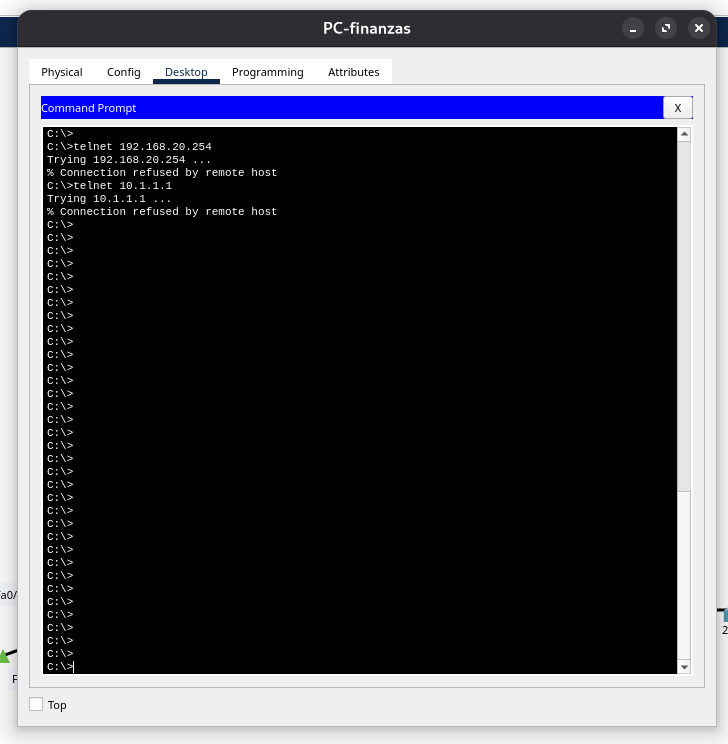
\includegraphics[scale=0.35]{imagenes/Capturas/22.png}
		\caption{Conexión desde PC-finanzas a un router (fallida)}
	\end{minipage}
	\hfill
	\begin{minipage}{0.45\textwidth}
		\centering
		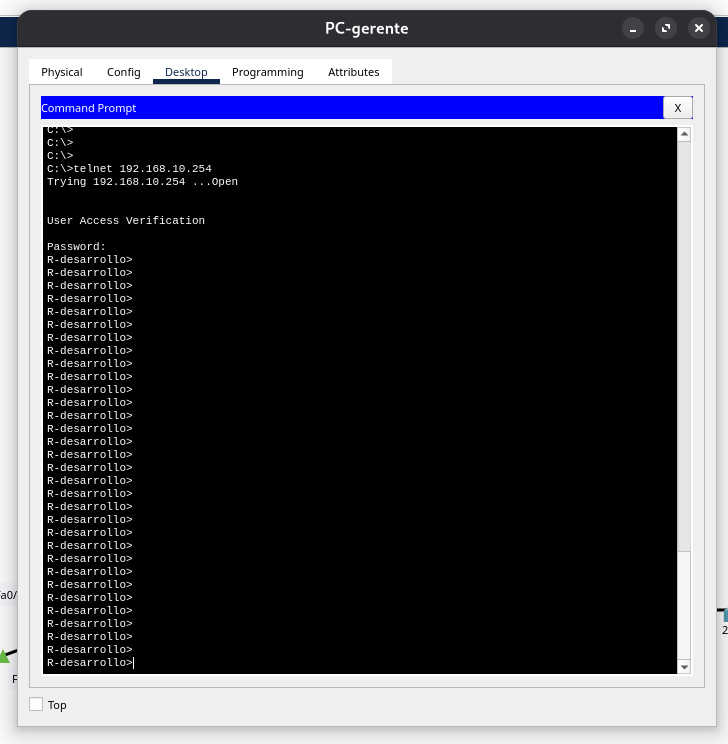
\includegraphics[scale=0.35]{imagenes/Capturas/23.png}
		\caption{Conexión desde PC-gerente a un router (exitosa)}
	\end{minipage}
\end{figure}

\subsection*{Los Servidores}
Entendí que todos los equipos de Finanzas (\texttt{192.168.20.0/24}) deben poder consultar páginas web (HTTP/HTTPS) y resolver nombres de dominio (DNS) alojados en la Red C (\texttt{192.168.30.0/24}). Sin embargo, Finanzas está usando comandos ping para jugar o saturar la red, por lo que el protocolo ICMP desde Finanzas hacia los Servidores debe ser bloqueado sin afectar su navegación web.

Aplicaremos una nueva ACL Extendida (120) en el router R-finanzas. Siguiendo la convención, la colocaremos lo más cerca posible del origen (interfaz Fa0/0), es decir en R-finanzas.
Permitiremos explícitamente los puertos UDP 53 (DNS), TCP 80 (HTTP) y TCP 443 (HTTPS). Luego, denegaremos el protocolo ICMP hacia la red \texttt{30.0} y, finalmente, permitiremos el resto del tráfico para no romper otras funciones del negocio.

\begin{lstlisting}[language=bash, numbers=none]
R-finanzas> enable
R-finanzas# configure terminal

- Permitimos resolución de nombres (DNS) de Finanzas a Servidores
R-finanzas(config)# access-list 120 permit udp 192.168.20.0 0.0.0.255 192.168.30.0 0.0.0.255 eq 53

- Permitimos navegación web (HTTP y HTTPS)
R-finanzas(config)# access-list 120 permit tcp 192.168.20.0 0.0.0.255 192.168.30.0 0.0.0.255 eq 80
R-finanzas(config)# access-list 120 permit tcp 192.168.20.0 0.0.0.255 192.168.30.0 0.0.0.255 eq 443

- Bloqueamos los pings (ICMP) de Finanzas hacia los Servidores
R-finanzas(config)# access-list 120 deny icmp 192.168.20.0 0.0.0.255 192.168.30.0 0.0.0.255

- Permitimos el resto del tráfico (para que Finanzas pueda salir a internet o al router central)
R-finanzas(config)# access-list 120 permit ip any any

- Aplicamos a la interfaz LAN de Finanzas
R-finanzas(config)# interface FastEthernet 0/0
R-finanzas(config-if)# ip access-group 120 in
R-finanzas(config-if)# exit
\end{lstlisting}

Probamos la configuración en Cisco Packet Tracer:
\begin{itemize}
	\item En PC-finanzas hacemos un ping a \texttt{192.168.30.200} (S-web).  Nos debe dar \textit{destination host unreachable}.
	\item Abrimos el Web Browser en PC-finanzas y entramos a \texttt{http://192.168.30.200} o \texttt{http://cripto.com}. Debe cargarse la página de Cisco.
\end{itemize}

\begin{figure}[H]
	\centering
	\begin{minipage}{0.3\textwidth}
		\centering
		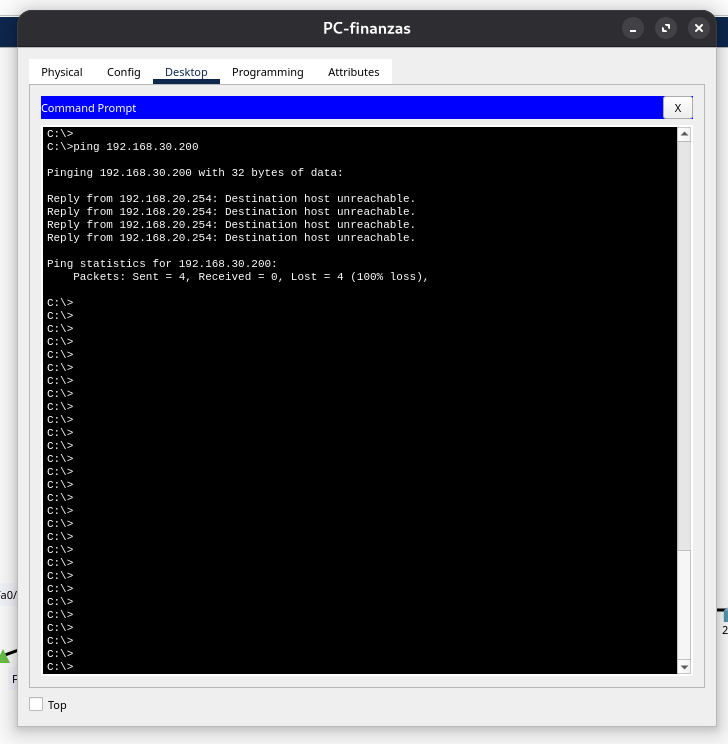
\includegraphics[scale=0.35]{imagenes/Capturas/31.png}
		\caption{Ping desde PC-finanzas al S-web (fallido)}
	\end{minipage}
	\hfill
	\begin{minipage}{0.45\textwidth}
		\centering
		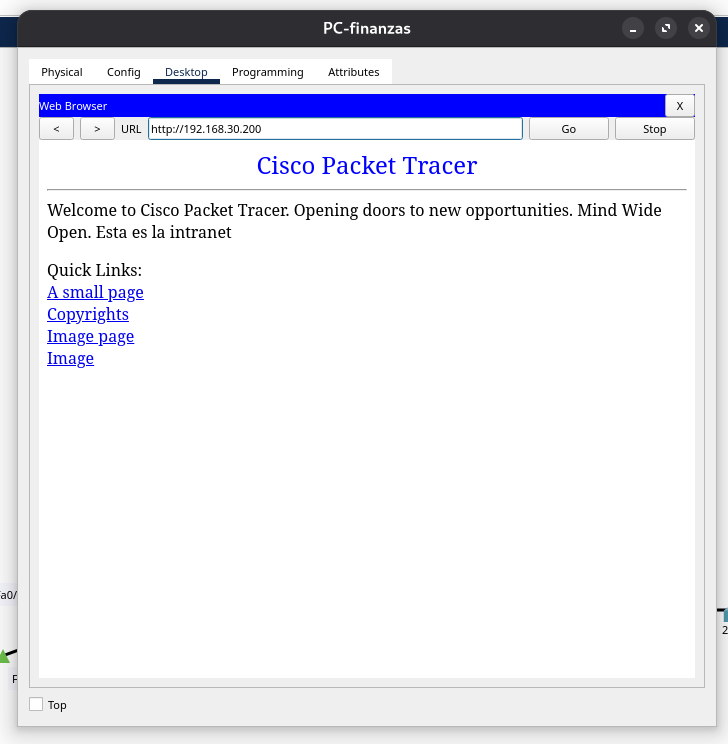
\includegraphics[scale=0.35]{imagenes/Capturas/32.png}
		\caption{Conexión HTTP desde PC-finanzas al S-web (exitosa)}
	\end{minipage}
\end{figure}

\subsection*{La puerta abierta de Desarollo}
Entendí que el equipo de Desarrollo (\texttt{192.168.10.0/24}) necesita acceso a DNS, Web y obligatoriamente a FTP (Transferencia de archivos) hacia la granja de servidores (\texttt{192.168.30.0/24}) para subir sus proyectos. El memorándum exige explícitamente cerrar todo lo demás hacia los servidores que no sea para su trabajo.

Ya tenemos la ACL 120 aplicada en la interfaz Fa0/0 de R-desarrollo, por lo cual la vamos a reestructurar. Agregaremos reglas que permitan los puertos de FTP (20 y 21), DNS (53) y HTTP/HTTPS (80/443). Luego, pondremos un \texttt{deny ip} de Desarrollo hacia Servidores para bloquear pings, telnet y cualquier otro servicio innecesario.

\begin{lstlisting}[language=bash, numbers=none]
R-desarrollo> enable
R-desarrollo# configure terminal

- Borramos la ACL actual para reordenarla correctamente
R-desarrollo(config)# no access-list 100

- Escribimos las reglas que hicimos antes)
R-desarrollo(config)# access-list 110 permit ip host 192.168.10.10 any
R-desarrollo(config)# access-list 110 permit tcp 192.168.10.0 0.0.0.255 192.168.20.0 0.0.0.255 established
R-desarrollo(config)# access-list 110 permit icmp 192.168.10.0 0.0.0.255 192.168.20.0 0.0.0.255 echo-reply
R-desarrollo(config)# access-list 110 deny ip 192.168.10.0 0.0.0.255 192.168.20.0 0.0.0.255

- Nuevas reglas hacia servidores
- Permitimos DNS
R-desarrollo(config)# access-list 110 permit udp 192.168.10.0 0.0.0.255 192.168.30.0 0.0.0.255 eq 53
- Permitimos Web
R-desarrollo(config)# access-list 110 permit tcp 192.168.10.0 0.0.0.255 192.168.30.0 0.0.0.255 eq 80
R-desarrollo(config)# access-list 110 permit tcp 192.168.10.0 0.0.0.255 192.168.30.0 0.0.0.255 eq 443
- Permitimos FTP (puerto 20 y 21)
R-desarrollo(config)# access-list 110 permit tcp 192.168.10.0 0.0.0.255 192.168.30.0 0.0.0.255 eq 21
R-desarrollo(config)# access-list 110 permit tcp 192.168.10.0 0.0.0.255 192.168.30.0 0.0.0.255 eq 20
- Denegamos todo lo demas de Desarrollo a Servidores
R-desarrollo(config)# access-list 110 deny ip 192.168.10.0 0.0.0.255 192.168.30.0 0.0.0.255

- Permitimos el resto del tráfico general a internet o cualquier otra red futura
R-desarrollo(config)# access-list 110 permit ip any any
R-desarrollo(config)# exit
\end{lstlisting}

Probamos la configuración en Cisco Packet Tracer:
\begin{itemize}
	\item En PC-dev y hacemos un ping a S-web (\texttt{192.168.30.200}). Debe ser bloqueado por la ACL.
	\item Abrimos el Command Prompt de PC-dev e intentamos transferir un archivo usando el protocolo FTP: \texttt{ftp 192.168.30.200}. Si todo está bien nos pedirá hacer login.
	\item Probamos el navegador web de PC-dev hacia \texttt{http://cripto.com}. Este debería cargar con normalidad.
\end{itemize}

\begin{figure}[H]
	\centering
	\begin{minipage}{0.3\textwidth}
		\centering
		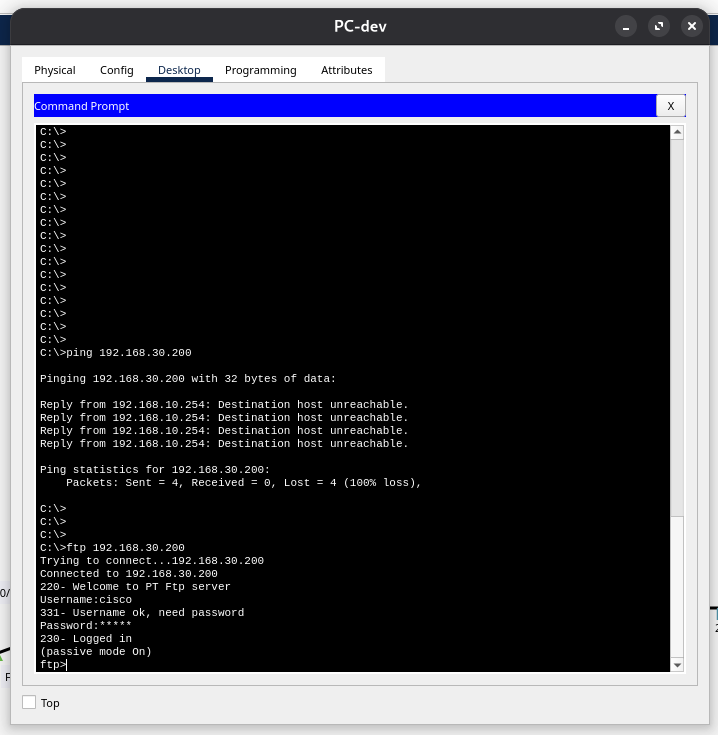
\includegraphics[scale=0.35]{imagenes/Capturas/41.png}
		\caption{Ping (fallido) y FTP (exito) desde PC-dev a S-web}
	\end{minipage}
	\hfill
	\begin{minipage}{0.45\textwidth}
		\centering
		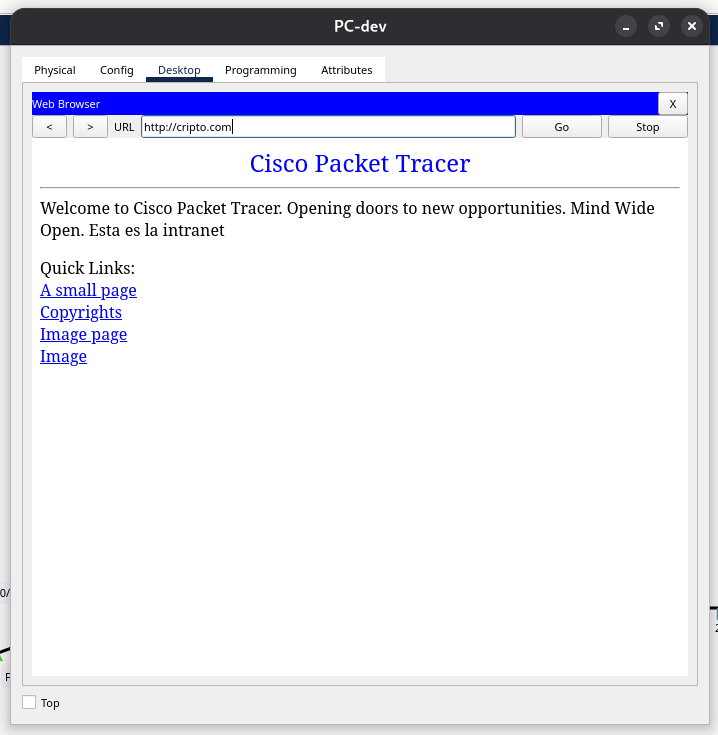
\includegraphics[scale=0.35]{imagenes/Capturas/42.png}
		\caption{Conexión HTTP desde PC-dev a S-web (exitosa)}
	\end{minipage}
\end{figure}